\chapter{Graph Denoising}
\label{sec:graphFoundations}
    

The following Chapter establishes connection between graphs and denoising in high-noise 
domains, such as cryo-EM.
First, a broad definition of graphs is given and further, the term "Graph Denoising" is
introduced and explained. Finally, link to Graph Laplacian, Manifolds and molecular imaging methods is established.

\section{Graph Foundations}
Real world data can be in graph structure, like social networks, citation networks,
protein interaction networks or a simple google search. 
If data is not available in graph structure, a graph can be artificially constructed with methods like k-nearest neighbors (k-NN) or others.
A general framework for graph construction is introduced in Section~\ref{sec:graphConstruction} \textit{\nameref{sec:graphConstruction}}.

\paragraph{Graph Learning:} Graph Learning is a prominent research area and got a lot of attention in recent years.
It is a way of applying ML on graphs and algorithms that have emerged emerged from ML but also other fields.
When a graph is available, one can start using Graph Learning algorithms for solving tasks.
Popular tasks are \textit{node classification} or \textit{link prediction}, where a model is learned from node and edge features 
as well as topology. The model can be used for prediction or classification on nodes or edges.
Another common task is \textit{community detection}, where the aim is to identify cluster of nodes within the input graph.
Further, graphs are highly favored for \textit{dimensionality-reduction}, where 
graph algorithms provide a helpful tool, as ordinary algorithms like principal component analysis fail to 
establish a meaningful dimensionality reduction.

\subsection{Graph definition}
A graph is defined as $G = \langle V,E \rangle$, where $V$ is a set of 
vertices (or nodes) and $E$ is a set of edges (or links). 
Edges are defined as a set of tuples $(i, j)$, where $i$ and $j$ determine 
the index of vertices in the graph.

\paragraph{Graph properties:}
A graph can be either \textit{directed} or \textit{undirected}. 
In a directed one, an edge connects explicitly from one node to another, which means that edge $(i, j) \neq (j, i)$. 
In undirected graphs, edges have no direction and ordering does not matter, therefore $(i, j) = (j, i)$.

The \textit{neighborhood}, denoted by $\mathcal{N}(i)$, of a node $i$  is defined as all adjacent nodes.
In other words, there is an edge between neighborhood nodes and $i$. 
Further, edges can have \textit{weights}, which is a method to define importance to neighbors, resulting in a \textit{weighted} graph.
\textit{Degree} of a node are the number of incoming edges.

\paragraph{Adjacency matrix:}
To do calculations with graphs, it is common to translate graphs in a matrix, 
such as the adjacency matrix.
The (binary) adjacency matrix of graph $G = \langle V, E \rangle$ is defined as follows:
\begin{equation}
    \label{eg:AdjacencyMatrix}
    A_{ij} =    
    \begin{cases}
        1  & \text{if } (i, j) \in E \\
        0, & \text{otherwise}
    \end{cases}
\end{equation}

Matrix $A$ has dimension $\mathbb{R}^{N \times N}$ with $N$ as number of nodes
and indices of $A$ correspond to nodes in $V$.
If there exists an edge between two nodes, entry in $A$ will be set to $1$, otherwise to $0$.
This leads to an unweighted graph, as weights of all edges will be $1$, 
but could easily be extended by assigned not just values of $1$ or $0$. 
When $G$ is undirected, corresponding adjacency matrix will be symmetric. 
Eigenvalues of $A$ are called \textit{spectrum} of $G$.


\subsection{Graph construction}
\label{sec:graphConstruction}
When data is not available as a graph, it can be easily constructed.
Consider data from space $\Omega \subset \mathbb{R}^M $, but could basically be any arbitrary space.
Then, each node is associated with some element $v \in \Omega$. 
Further, graph $G$ can be constructed by using:

\begin{equation}
    \label{eq:graphConstruction}
    A_{ij} =    
    \begin{cases}
        1  & \text{if } dist(v_i, v_j) < \tau\\
        0, & \text{otherwise}
    \end{cases}
\end{equation}

where $v_i$, $v_j$ are nodes from indices $i$ and $j$, $dist$ corresponds to a similarity (or distance) measure and $\tau$ is a threshold, 
when to consider two nodes to be adjacent.
K-NN is one possible implementation of a graph construction algorithm, 
where for every node, $k$ neighbors will be defined.
The neighborhood $\mathcal{N}_i$ of $v_i$ is defined as $k$ nodes with the smallest similarity measure.

\paragraph{Noisy observations:}
But what happens if our data is noisy?
Consider measurements which will give access to $y = p + \eta$, where $y,p \in \Omega$ and noise $\eta$ is assumed to be drawn from Gaussian distribution $\mathcal{N} \sim (0,\sigma^2)$.
$y$ refers to the noisy observation and $p$ to noiseless observation.
While constructing a graph, nodes are associated with elements from $p$ ($dist(p_i, p_j)$) in the noiseless case and from $y$ ($dist(y_i, y_j)$) is the noisy case.
Therefore, k-NN applied on noisy data, is assumed to connect some nodes wrongly, as distance measure $dist$
is not accurate due to noise. It is expected that the more noise is available in data, the more nodes are wrongly connected with k-NN.

\paragraph{Constructing Graphs for molecular-imaging:}
For a molecular-imaging (cryo-EM or computed tomography) observation, a graph can be constructed as well.
Every observation $y_i$ can be assigned to a node $v_i$, which means that $V \subset \mathbb{R}^M$, where 
$M$ is again observation dimension. 
Further, $|V|=N$ where $N$ is the number of observations, which defines how many projections from different
angles $\theta$ are within the observation.

Finally, to apply Equation~\ref{eq:graphConstruction} similarity measure $dist$ needs to be defined.
For computed tomography, a distance measure between observations can be set up by using the $\ell2$-norm $\norm{y_i - y_j}$.
For cryo-EM it is more challenging, as projections are drawn with some random 3D rotation and projection, 
it can happen that two samples are equivalent up to 2D rotation. 
Consider a first observation $y_1$, which has no 3D rotation and 
a second observation $y_2$ with a rotation in x-y plane by 45°.
The two projections have a defined in-plane rotation $g$, such that $g \; y_1 = y_2$.
Therefore, a term of in-plan rotation is added to the $\ell2$-norm: $min_{g \in SO(1)}\norm{g \;y_i - y_j}$, 
which is inspired by \cite{multiDiffusionMaps}. 

Now, everything is available to create a graph from a molecular-imaging observation.


\section{Graph Denoising definition}

First, \textit{Graph Denoising} is not a common term in literature.
In previous Section, graphs based on noisy observations were introduced and goal is to denoise these graphs,
which means to estimate original graph $G$ from a given noisy graph $G_0$. 
This is our definition for Graph Denoising, which is rather related to signal or image denoising.
Reconstruction of a true signal given noisy observation signal is done via averaging, that can be performed
locally, by the calculus of variations or in the frequency domain~\cite{noneLocalMean}. 

\paragraph{Noisy Graph:}
For every noisy graph there exists an original graph $G = \langle V,E \rangle$.
The noisy graph $G_0$ can further be defined as $G_0 = \langle V, E_0 \rangle$,  
 where $E_0 = E \setminus  E^{-}_0 \cup  E^{+}_0$ with $E^{-}_0 \subseteq E$ and $E^{+}_0 \cap E = \emptyset$.

$G_0$ consists of same nodes $V$ as original graph $G$. 
From $E$ some edges are removed (denoted by $E^{-}_0$) and some are added
(denoted by $E^{+}_0$), which results in edges $E_0$.

Graph Denoising can therefore be written as 
\begin{equation}
    GD: A_0 \mapsto \tilde{A} \approx A
\end{equation}

where $A_0$, $\tilde{A}$, $A$ denotes adjacency matrix from noisy input graph, denoised graph and original graph respectively.


\paragraph{Connection to link prediction:}
Link prediction is a task in Graph Learning. 
The goal is to predict existence of a link between two nodes.
The task can be formulated as a missing value estimation task. A model $M_p$ is learned
from a given set of observed edges. The model finally maps links to probabilities
$M_p : E^{\prime} \rightarrow [0,1]$ where $E^{\prime}$ is the set of potential links.

Further, $U$ determines the set of all possible vertices of $G$, therefore $E \subseteq U$.
Clearly, Graph Denoising can be seen as a link prediction problem.
The difference is, that in link prediction a model from a set of observed links is learned
$E^{\prime} \subseteq E$ and in Graph Denoising model is learned from 
$E^{\prime} \subseteq U$. 

\begin{tcolorbox}[colback=red!5!white,colframe=red!75!black]
    One could also say that link prediction problems are a subset of graph denoising problems.
\end{tcolorbox}

\paragraph{Non-local means:}
In the following Section, a short introduction to the 
state-of-the-art image denoising method non-local means (NLM)~\cite{noneLocalMean} is given .
For a given noisy image $v$, the denoised image is defined as $NL[v](i) = \sum{w(i,j) \; v(j)}$,
where $w(i,j)$ is the weight between pixel $i$ and $j$. 
Weights can be seen as a similarity measure of pixels, which are calculated over square neighborhoods.
Similar pixel neighborhoods have a large weight and different neighborhoods have a small weight.
More general, denoised image pixel $i$ is computed as a weighted average of all pixels in the 
image, therefore, in a non-local way.

Non-local means is not a denoising algorithm, which works with graph as a data structure.
But, it uses a neighborhood for averaging, which shows great potential for graph
as a data structure for denoising, as graphs can represent neighborhoods really well.


\section{Graph Deep Learning}
\label{sec:graph_depp_learning}
As already mentioned, Graph Denoising can be seen as a way of link predication. 
The state-of-the-art method for solving link prediction are \textit{Graph Deep Learning} approaches.
Graph Deep Learning is a fast evolving field in research. With Graph Neural Networks (GNN)~\cite{GNN} the framework
for neural networks with graphs has been established. 

Using Graph Convolutional Networks (GCN)~\cite{GCN} for graph feature extraction is a popular way. 
With GCN a new feature representation is iteratively learned for node features (edge features are not considered).
It can be seen as an averaging of nodes over their neighborhood where all neighbors get the same weight combined with some non-linear activation (e.g. ReLu). 
To consider node itself in averaging, \citet{GCN} applies the so-called "Renormalization trick", where self-loops are added to the 
adjacency matrix and after every layer, a normalization step is applied. 
The topology of the graph will not be adjusted during learning process.

\citet{GAT} extended the concept of GCN with attention and not all neighboring nodes get the same weight (attention).
Simple Graph Convolutional Network~\cite{simpleGCN} proposed a simplified version of GCN.
They could verify their hypothesis that GCN is dominated by local averaging step and non-linear 
activation function between layers do not contribute too much to the success of GCN. 
Therefore, it can be seen as a way of power iteration (see \ref{sec:powerIterations} \textit{\nameref{sec:powerIterations}} for further information) over the adjacency matrix with normalization in every layer.
\citet{dynamicGCN} proposed an extension to GCN by not operating on the same graph in every layer but adopting
underlying graph topology layer by layer.

\section{Graph Laplacian \& Manifolds}
\subsection{Graph Laplacian}
Graph Laplacian (GL) is a matrix that represents a graph and can be used to find many important properties.
It is a very powerful tool and a good introduction and overview can be found by \cite{tutorialSpectralClustering, SpectralGraphTheory}. 

GL is defined as follows:
\begin{equation}
    \label{eq:gl}
    L = D - A,
\end{equation}

where $A$ is the adjacency matrix and $D$ the degree matrix (diagonal matrix with degree of nodes as entries).

\subsection{Manifolds}
\label{sec:manifolds}

In high-dimensional data Euclidean distances are not meaningful
in the sense that they will not capture similar data points well. One is looking for a geodesic distance, 
representing the shortest path of two point on a surface.
Graph Laplacian can be used to compute a \textit{Manifold}, which can help in such scenarios. 
In manifold space, Euclidean distances make sense again. 
Let manifold $M$ be defined as $\mathcal{M} = \{ f(x), f \in C^K, f: \mathbb{R}^D \to \mathbb{R}^d \}$.
Manifolds are a well established mathematical concept. In the Master's Thesis, only 
$C^k$ differentiable d-dimensional manifolds defined by $\mathcal{M}$ are considered. 
When $d \ll D$, manifolds define a \textit{low-dimensional embedding}, which maps from high-dimensional space 
$\mathbb{R}^D$ to low-dimensional space $\mathbb{R}^d$.

Let's give two popular examples of manifolds, namely \textit{circle} and \textit{sphere}.
The circle is a 1D manifold, where $d=1$ and $D=2$. A sphere is a 2D manifold, with $d=2$ and $D=3$.
In Figure~\ref{fig:circle_sampling}, 200 samples are drawn from a uniform distribution of unit-circle manifold
and in Figure~\ref{fig:sphere_sampling}, 800 samples are drawn from a uniform distribution of unit-sphere manifold,
as well as the sphere itself.

\begin{figure}[H]
    \hfill
    \subbottom[
        \label{fig:circle_sampling}]
        {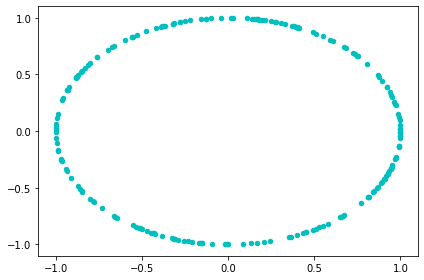
\includegraphics[width=0.4\textwidth]{circle_sampling.png}}
    \hfill
        \subbottom[      
    \label{fig:sphere_sampling}]
        {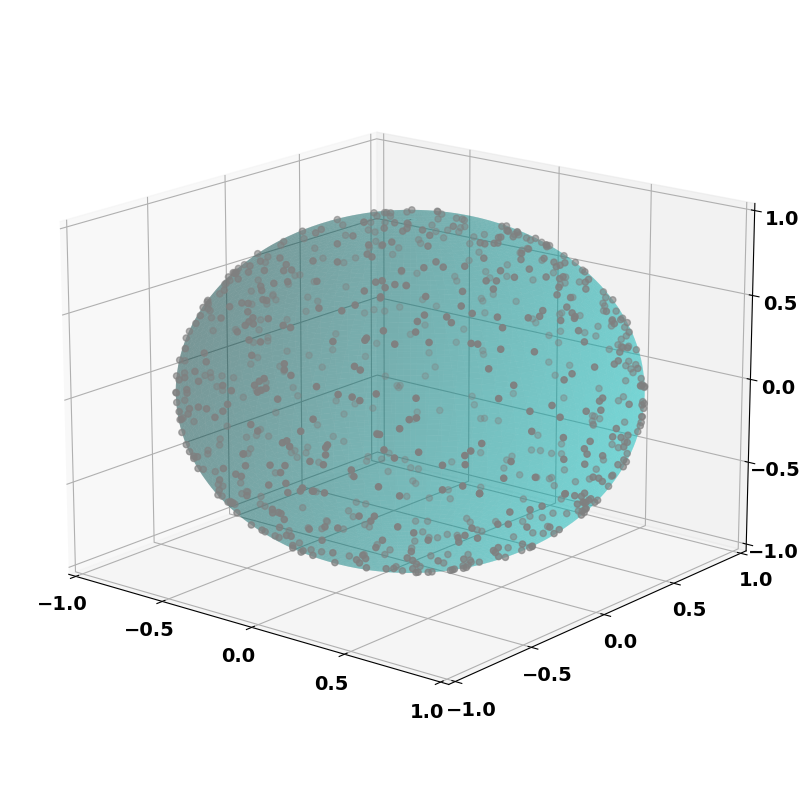
\includegraphics[width=0.42\textwidth]{sphere_sampling.png}}
    \hfill
        \caption{Samples drawn from 1D and 2D manifold: 
    \ref{fig:circle_sampling} circle samples,
    \ref{fig:sphere_sampling} sphere samples}
\end{figure}

One popular algorithm for calculating manifolds is diffusion maps~\cite{diffusionMaps}, 
which is a non-linear approach for calculating low-dimensional manifolds
for (high-dimensional) datasets, using Graph Laplacian.
Vector diffusion maps~\cite{vectorDiffusionMaps} generalize the concept of diffusion maps for vector fields.
Multi-frequency vector diffusion maps~\cite{multiDiffusionMaps} 
can be seen as an extension to vector diffusion maps, which works well even on highly noisy environments.
\citet{cryoEmMutliDM} successfully applied multi-frequency vector diffusion Maps in cryo-EM setting,
 where it was used for denoising purpose.

\subsection{Manifold assumption}
\label{sec:manifoldAssumption}
Manifold assumption is a popular assumption for high-dimensional datasets.
For a given dataset in high-dimension, one can assume that data points are samples drawn from a low-dimensional manifold,
that embeds the high-dimensional space. 
Therefore, if underlying manifold can be approximated, a dimensionality reduction
is established as one can embed data points in the low-dimensional manifold space.
There is a complete area of research devoted to this manifold assumption called Manifold Learning\cite{ManifoldLearning}.

\subsection{GL-manifold calculation}
\label{sec:manifold_calculation}
A simple low-dimensional embedding (manifold) of a dataset can be calculated with Graph-Laplacian 
by the following:

\begin{enumerate}
    \item Construct k-NN graph from observations (see Section~\ref{sec:graphConstruction} \textit{\nameref{sec:graphConstruction}}).
    \item Calculate the (normalized) Graph Laplacian (see Equation~\ref{eq:gl}).
    \item Extract the second, third (and fourth) the smallest eigenvectors.
\end{enumerate}

\subsection{Manifold of computed tomography and cryo-EM}
\label{sec:manifold_ct_cryoEM}
As a tool for GL-manifold calculation is established, it can be observed how the GL-manifold of classical tomography and cryo-EM objects look like.
In the following, Shepp-Logan phantom is again used as an example of classical tomography
and the low-dimensional embedding is calculated from sinogram, following instructions from 
Section~\ref{sec:manifold_calculation} \textit{\nameref{sec:manifold_calculation}}.

Radon Transform, parameters $\theta$ and $s$ where specified as $\theta \in \mathbb{R}^{500}$ as evenly spaced
between $[0, 2 \pi]$ and $dim(s) = 200$. 

In Figure~\ref{fig:clean_manifold}, GL-manifold calculated from clean sinogram and $k=2$ can be seen.
GL-manifold looks like a perfect circle. Further, noise was added to the sinogram 
to reach SNR 20dB and GL-manifold was computed with $k=2$, which failed (figure~\ref{fig:noisy_manifold_k2}).
But, if neighborhood is not too strictly defined and k is increased to 4, GL-manifold looks more circle like again
(figure~\ref{fig:noisy_manifold_k4}).

\begin{figure}[H]
    \centering
    \hfill
    \subbottom[\label{fig:clean_manifold}]
        {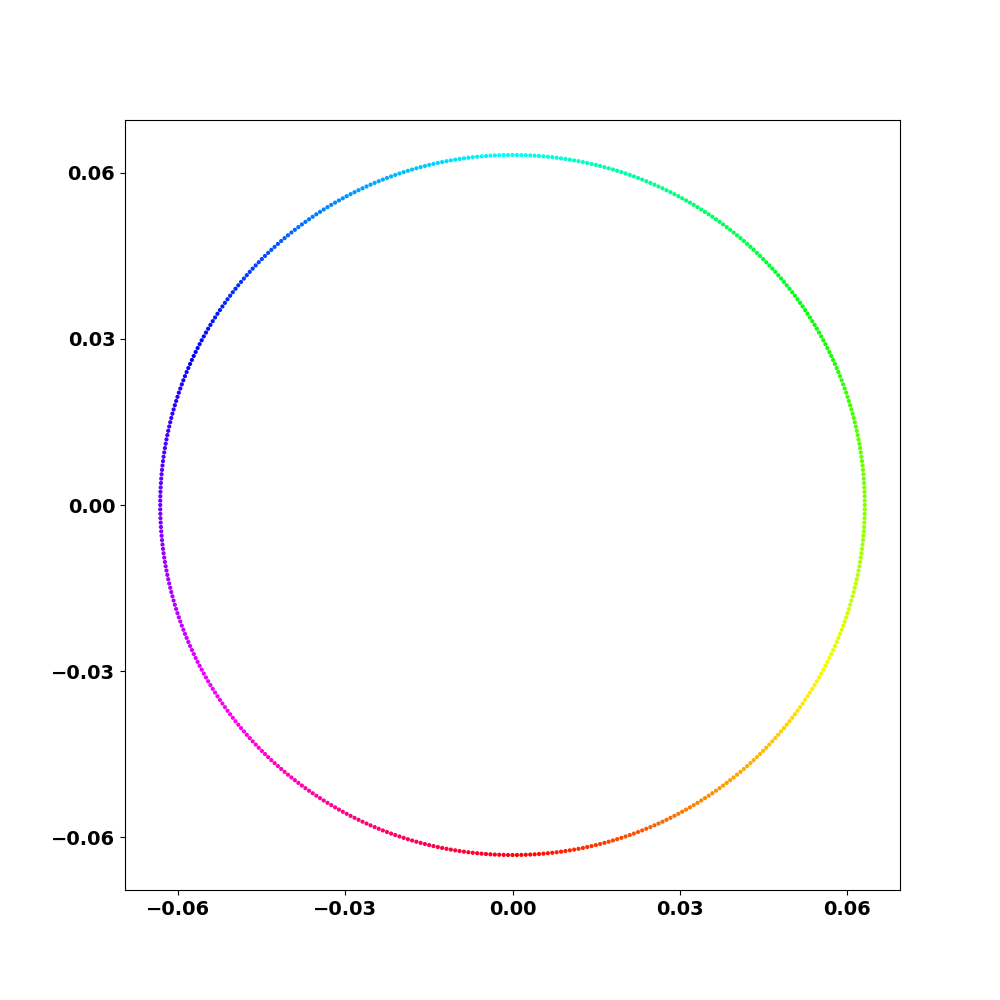
\includegraphics[width=0.3\textwidth]{phaton_clean_manifold.png}}
        \hfill
    \subbottom[\label{fig:noisy_manifold_k2}]
        {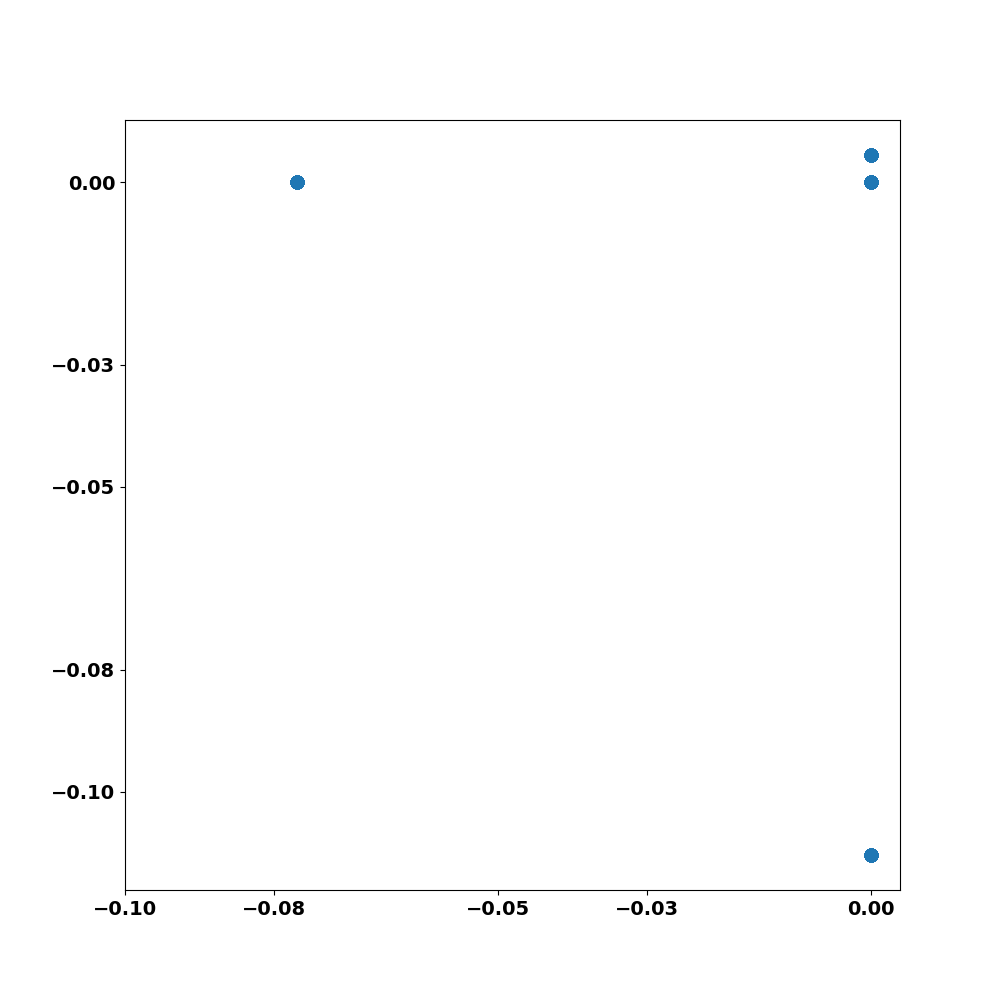
\includegraphics[width=0.3\textwidth]{phaton_noisy_manifold_k2.png}}
    \hfill
    \subbottom[\label{fig:noisy_manifold_k4}]
            {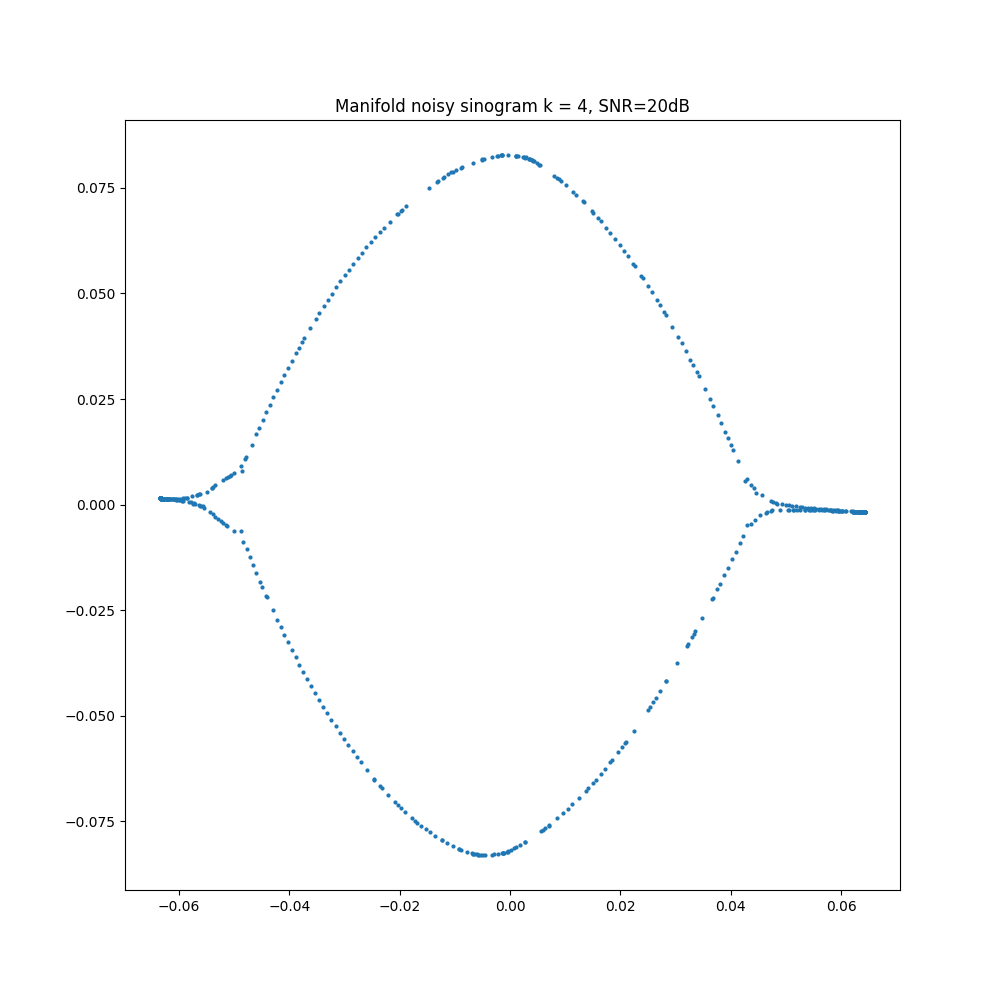
\includegraphics[width=0.3\textwidth]{phaton_noisy_manifold_k4.png}}
    \hfill
    \caption{Shepp-Logan phantom sinogram manifolds:
    \ref{fig:clean_manifold} clean sinogram manifold $k=2$,
    \ref{fig:noisy_manifold_k2} noisy sinogram manifold $k=2$,
    \ref{fig:noisy_manifold_k4} noisy sinogram manifold $k=4$
    }
\end{figure}

\begin{tcolorbox}[colback=red!5!white,colframe=red!75!black]
    In the field of classical tomography and cryo-EM, underlying low-dimensional GL-manifold is well-defined for none-noisy data.
    In the 2D case of classical tomography, underlying GL-manifold is a circle, whereas in 3D case of cryo-EM  GL-manifold
    is defined as a sphere.
    This fact can be exploited during learning.
\end{tcolorbox}

\paragraph{Manifold quality:}

Finding a good GL-manifold is not easy and in our case, GL-manifold is dependent on parameter $k$ during graph construction
as well as parameter $\theta$, $s$ and $\eta$ for obtaining the sinogram.

K is an important parameter for building up a graph. If set too low, neighbors
do not capture similar data well as too few nodes are connected. 
Further, if k is set too high, strength of a neighbor 
is weakened and data is not well explained as well.
In Figure~\ref{fig:clean_manifolds}, GL-manifold computed by clean sinogram and k from 2 to 10 is illustrated.
One can see, that from $k <= 4$ GL-manifold results in a perfect circle and with $k >  4$ is moves 
further away from the circle. 


\begin{figure}[H]
    \centering
    \hfill
    \subbottom[\label{fig:clean_manifolds}]
        {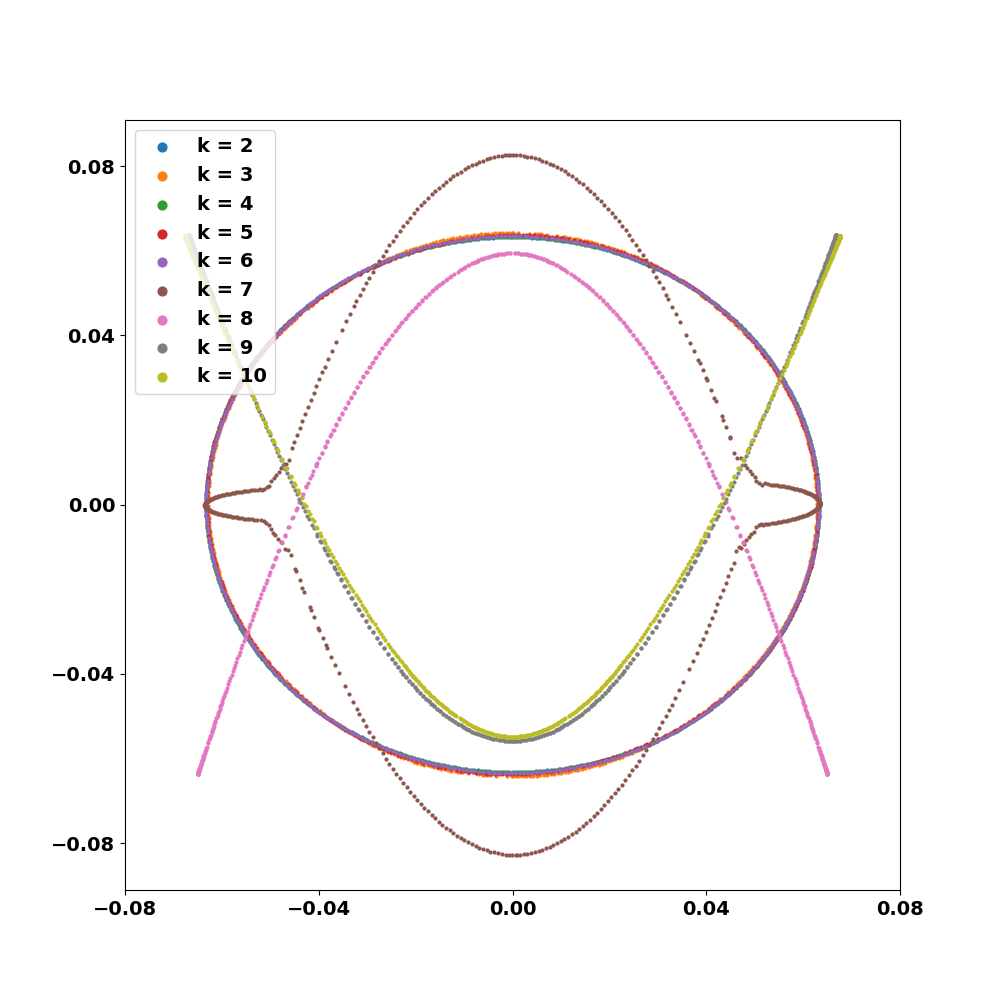
\includegraphics[width=0.45\textwidth]{phaton_clean_manifold_kdifferent.png}}
    \hfill
    \subbottom[\label{fig:noisy_manifolds}]
        {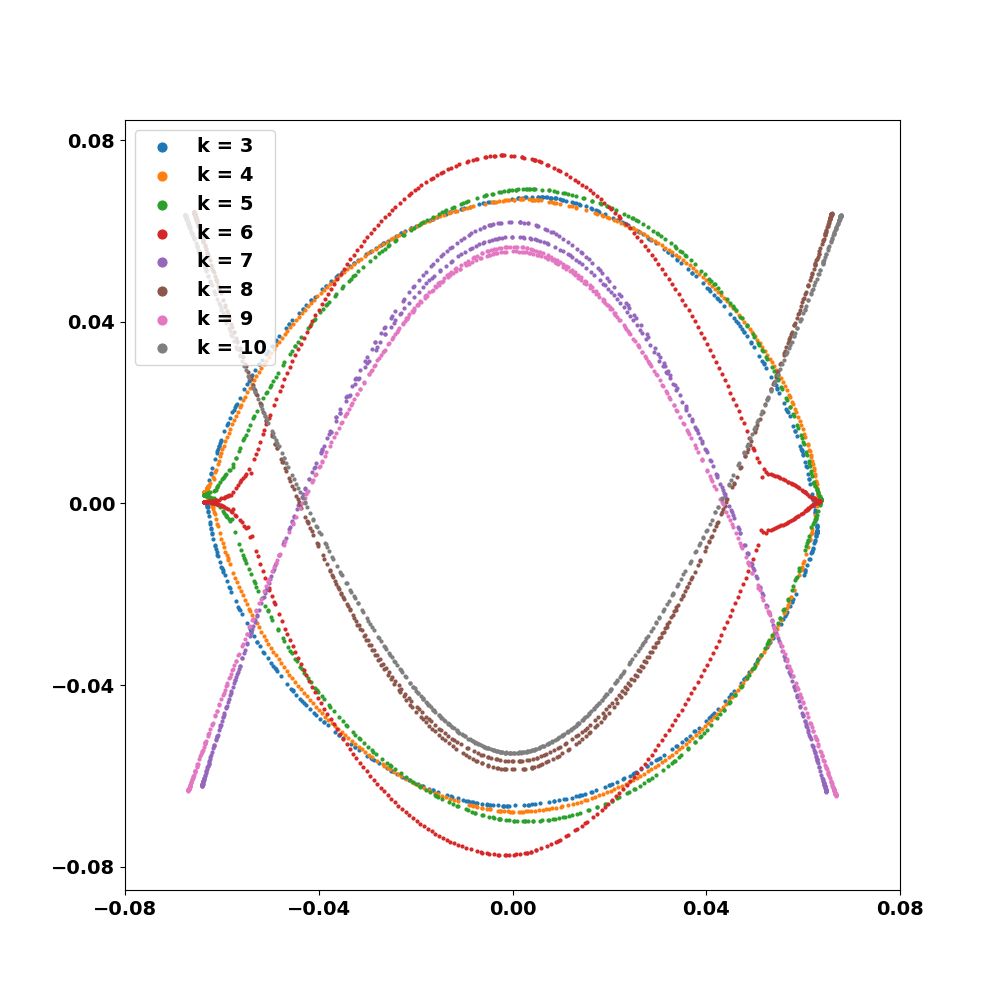
\includegraphics[width=0.45\textwidth]{phaton_noisy_manifold_kdifferent.png}}
    \hfill
    \caption{Shepp-Logan phantom sinogram manifolds:
    \ref{fig:clean_manifolds} clean sinogram GL-manifolds,
    \ref{fig:noisy_manifolds} noisy sinogram GL-manifolds}
\end{figure}

If data is noisy, it is expected to be harder to construct a meaningful GL-manifold, as some connections within
the graph will be noisy. This is exactly what is illustrated in Figure~\ref{fig:clean_manifolds}, where 
different GL-manifold for noisy sinogram (SNR=20dB) and k from 3 to 10 are illustrated.
GL-manifold can never express the true data with a perfect circle. As noise is chosen rather moderate, GL-manifold has still some 
power to express underlying data and is expected to decrease, if noise is increased.


Further, when observing a sinogram, parameter $\theta$ defines how many observations (straight lines) are drawn
and $dim(s)$ defines the amount of sampling points. Both have great impact to expressiveness of our sinogram.

\begin{figure}[H]
    \centering
    \hfill
    \subbottom[\label{fig:clean_manifold_200}]
        {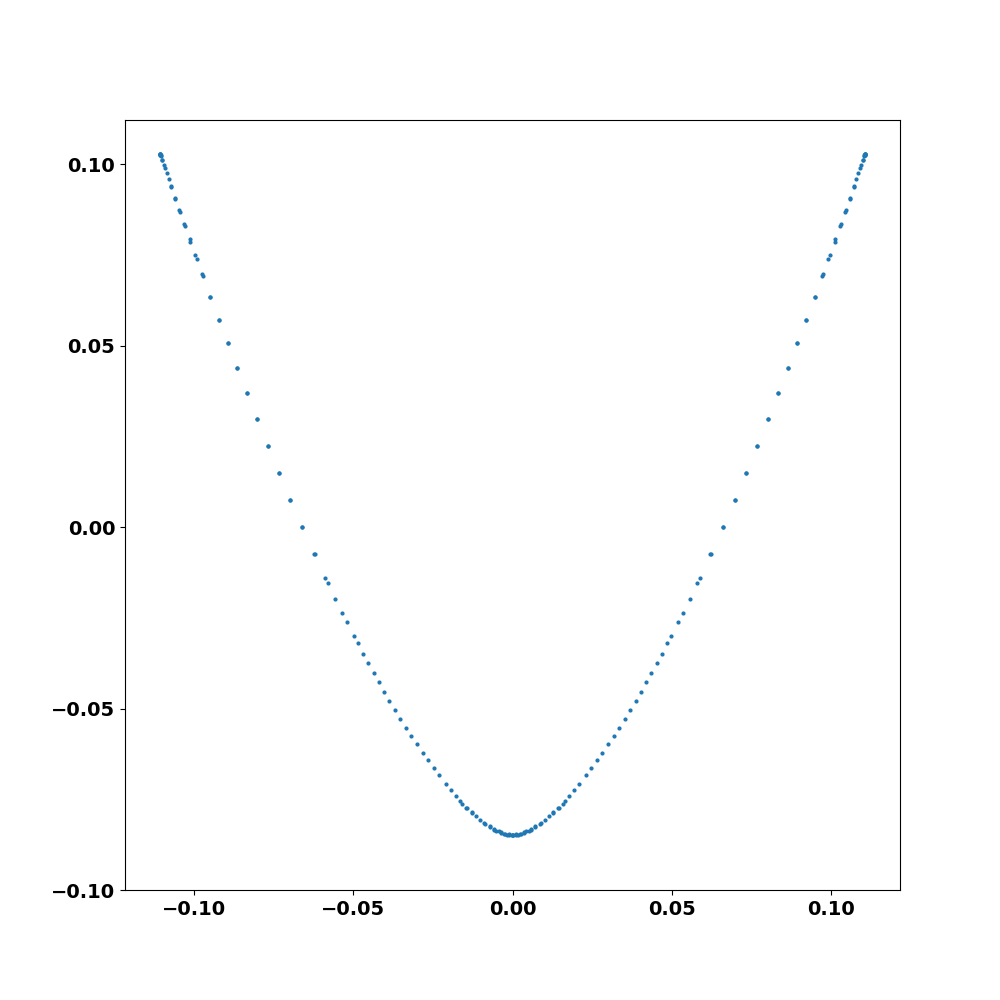
\includegraphics[width=0.3\textwidth]{phaton_clean_manifold_200_k6.png}}
    \hfill
    \subbottom[\label{fig:clean_manifold_500}]
        {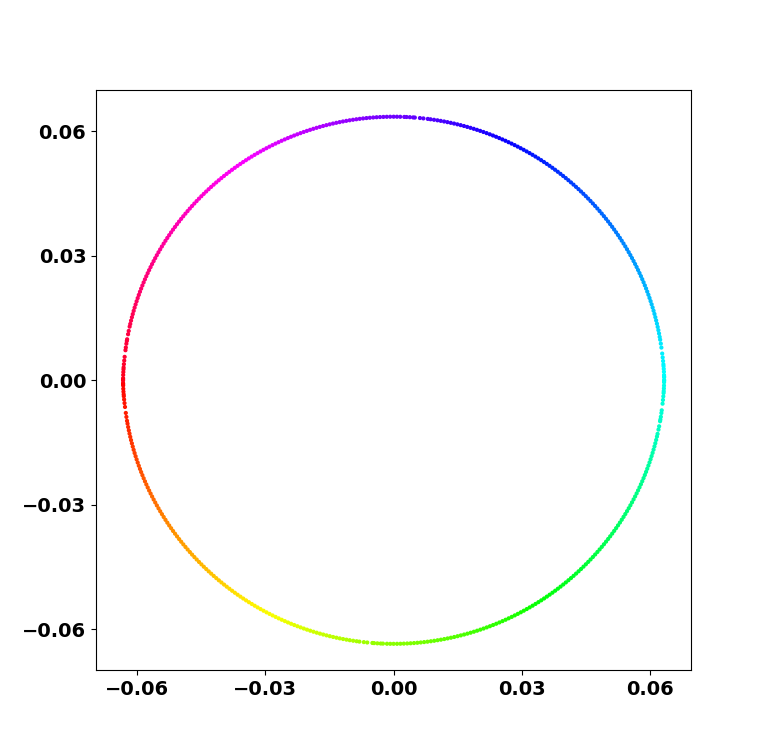
\includegraphics[width=0.3\textwidth]{phaton_clean_manifold_500_k6.png}}
    \hfill
    \caption{Shepp-Logan phantom sinogram GL-manifolds: Importance of number of samples.
    \ref{fig:clean_manifold_200} clean sinogram GL-manifold, $k = 6$ and 200 samples,
    \ref{fig:clean_manifold_500} clean sinogram GL-manifold, $k = 6$ and 500 samples}
\end{figure}

In Figure~\ref{fig:clean_manifold_200} GL-manifold with $\theta \in \mathbb{R}^{200}$ and k=6 is illustrated
for clean sinogram. It looks like 6 are too many neighbors, as the perfect circle cannot be established anymore.
But, if $\theta$ is increased $\theta \in \mathbb{R}^{500}$, more nodes are available to choose good neighbors from
and a perfect circle can be established (figure~\ref{fig:clean_manifold_500}).

\begin{figure}[H]
    \centering
    \hfill
    \subbottom[\label{fig:clean_manifold_res200}]
        {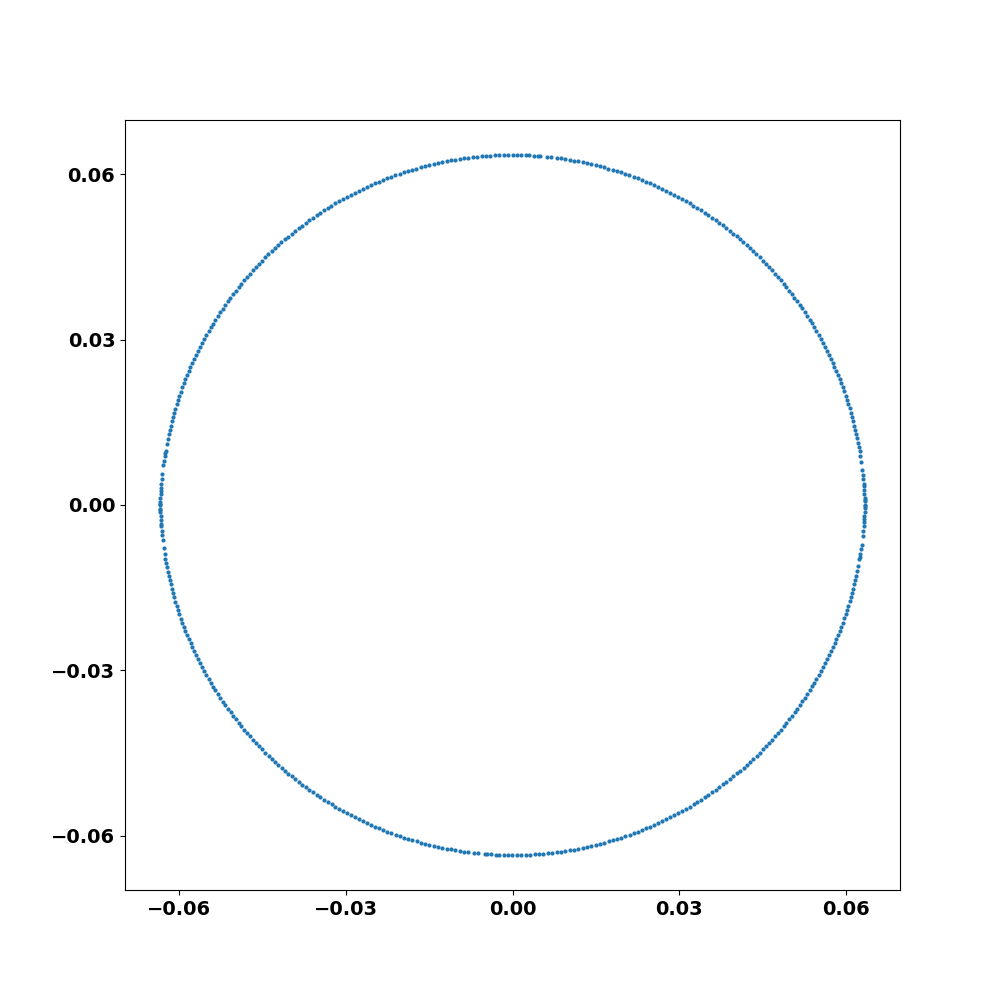
\includegraphics[width=0.3\textwidth]{phaton_clean_manifold_res_200_k6.png}}
    \hfill
    \subbottom[\label{fig:clean_manifold_res400}]
        {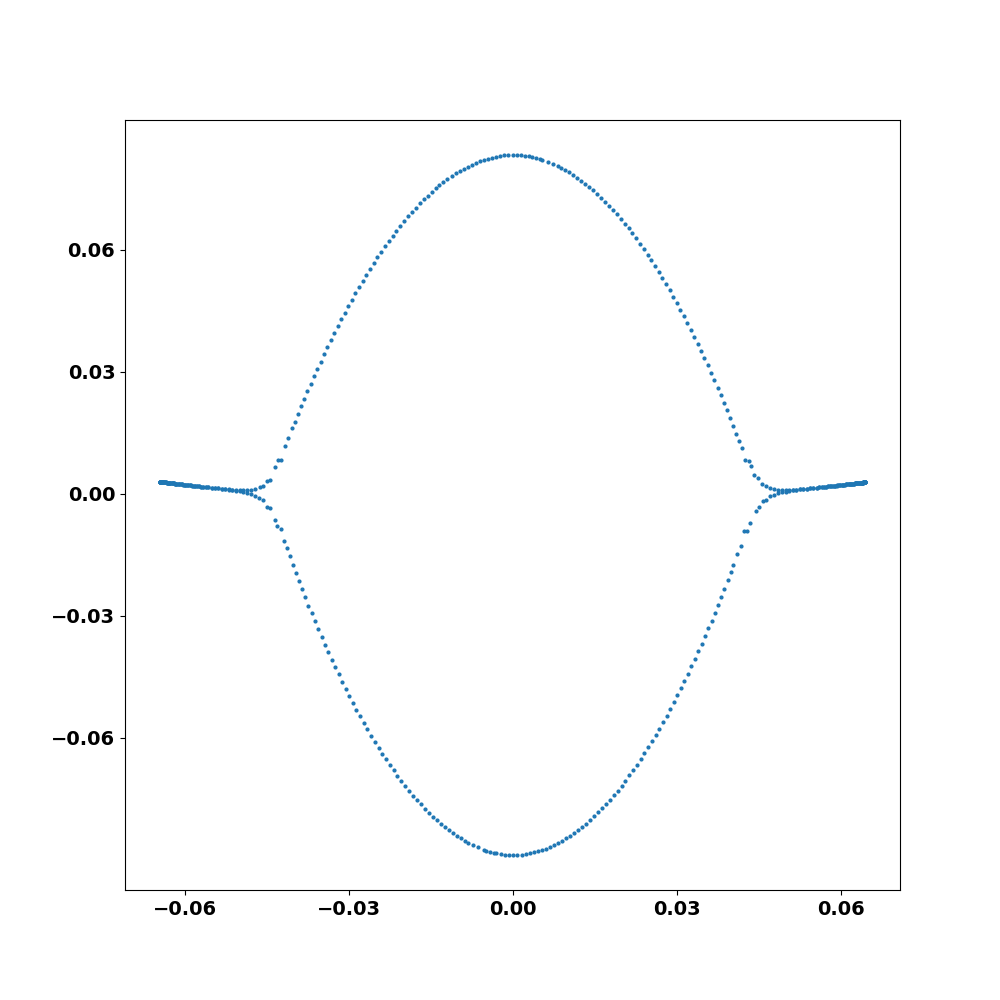
\includegraphics[width=0.3\textwidth]{phaton_clean_manifold_res_400_k6.png}}
    \hfill
    \caption{Shepp-Logan phantom sinogram GL-manifolds: Importance of number of samples.
    \ref{fig:clean_manifold_res200} Clean sinogram GL-manifold, $k = 6$ and $\text{resolution}=200$,
    \ref{fig:clean_manifold_res400} Clean sinogram GL-manifold, $k = 6$ and $\text{resolution}=400$}
\end{figure}

Moreover, the number of sampling points is important as well.
Here, for more sampling points it is expected to be harder to come up with good neighbors (fixing k and number of samples),
as more data need to be explained with the same amount of neighbors, and it is more likely, that nodes are connected wrongly.
This can be seen in Figure~\ref{fig:clean_manifold_res200} and Figure~\ref{fig:clean_manifold_res400}, where with $dim(s) = 200$,
the perfect circle can be established and with $dim(s) = 400$, not anymore (by same parameter $k = 6$ and $\theta \in \mathbb{R}^{500}$).

\begin{tcolorbox}[colback=red!5!white,colframe=red!75!black]
    As with the last plots illustrated, the GL-manifold is pretty sensitive.
    Therefore, it is best practice to try different parameter $k$ for finding the best 
    GL-manifold.
\end{tcolorbox}



\textbf{TODO: Connection to next chapter}